\chapter{Digital Flow}
\label{chapter:digital-flow}

The goal of this chapter is to present an evolution process that decreases digital elastica energy and can be used in practice. In particular, an application in image segmentation is presented at the end of the chapter. 

\section{Potential elastica}

As observed in the previous chapter, a global optimization model is unlikely to be useful in practice. In this section, we are going to explore the definition of the II estimator to derive a process that evolves the shape $S$ based on measurements of its current boundary $\partial S$. We start by defining a naive energy that illustrates some of the issues with this approach and how we can overcome them.

As usual, let $S \in \Omega \in \mathbb{Z}^2$ be a digital shape. We assume an ordering in $\Omega$, i.e., there exists a bijective function $\omega : \Omega \rightarrow \{1 \cdots |\Omega| \}$. Moreover, we associate to any subset $P \subset \Omega$ the set of binary variables $X(P)$ defined as

\begin{align*}
	X(P) := \left\{ x_{\omega(p)} \in \{0,1\} \; | \; p \in P \right\}.
\end{align*}

\begin{definition}{Inner pixel boundary}
Given a digital shape $S \in \Omega \in \mathbb{Z}^2$, we define its inner pixel boundary set $I(S)$ as
\begin{align*}
	I(S) := \left\{ \: p \; | \; p \in S, |\mathcal{N}_4(x) \cap S|<4 \: \right\},
\end{align*}
where $\mathcal{N}_4(p)$ denotes the $4$-adjacent neighbor set of $p$ (without $p$).
\end{definition}


We recall the II estimator definition

\begin{align*}
	\hat{k}(p) = \frac{3}{r^3}\left( \frac{\pi r^2}{2} - |B_r(p) \cap S| \right).
\end{align*}

Consider the following optimization problem and its result for the square shape with parameters $h=0.5,r=10$ in figure \ref{}.

\begin{align}
	\min_{X(I(S)} \sum_{p \in I(S)}{ \Big( \; \frac{\pi r^2}{2} - | (B_r(p) \cap S) \setminus I(S) | - \sum_{ \substack{x_j \in \\ X( I(S) \cap B_r(p))}}{x_j} \; \Big)^2}.
	\label{eq:naive-opt-problem}
\end{align}

\begin{figure}
\center
\subfloat[\label{fig:naive-opt-before}]{
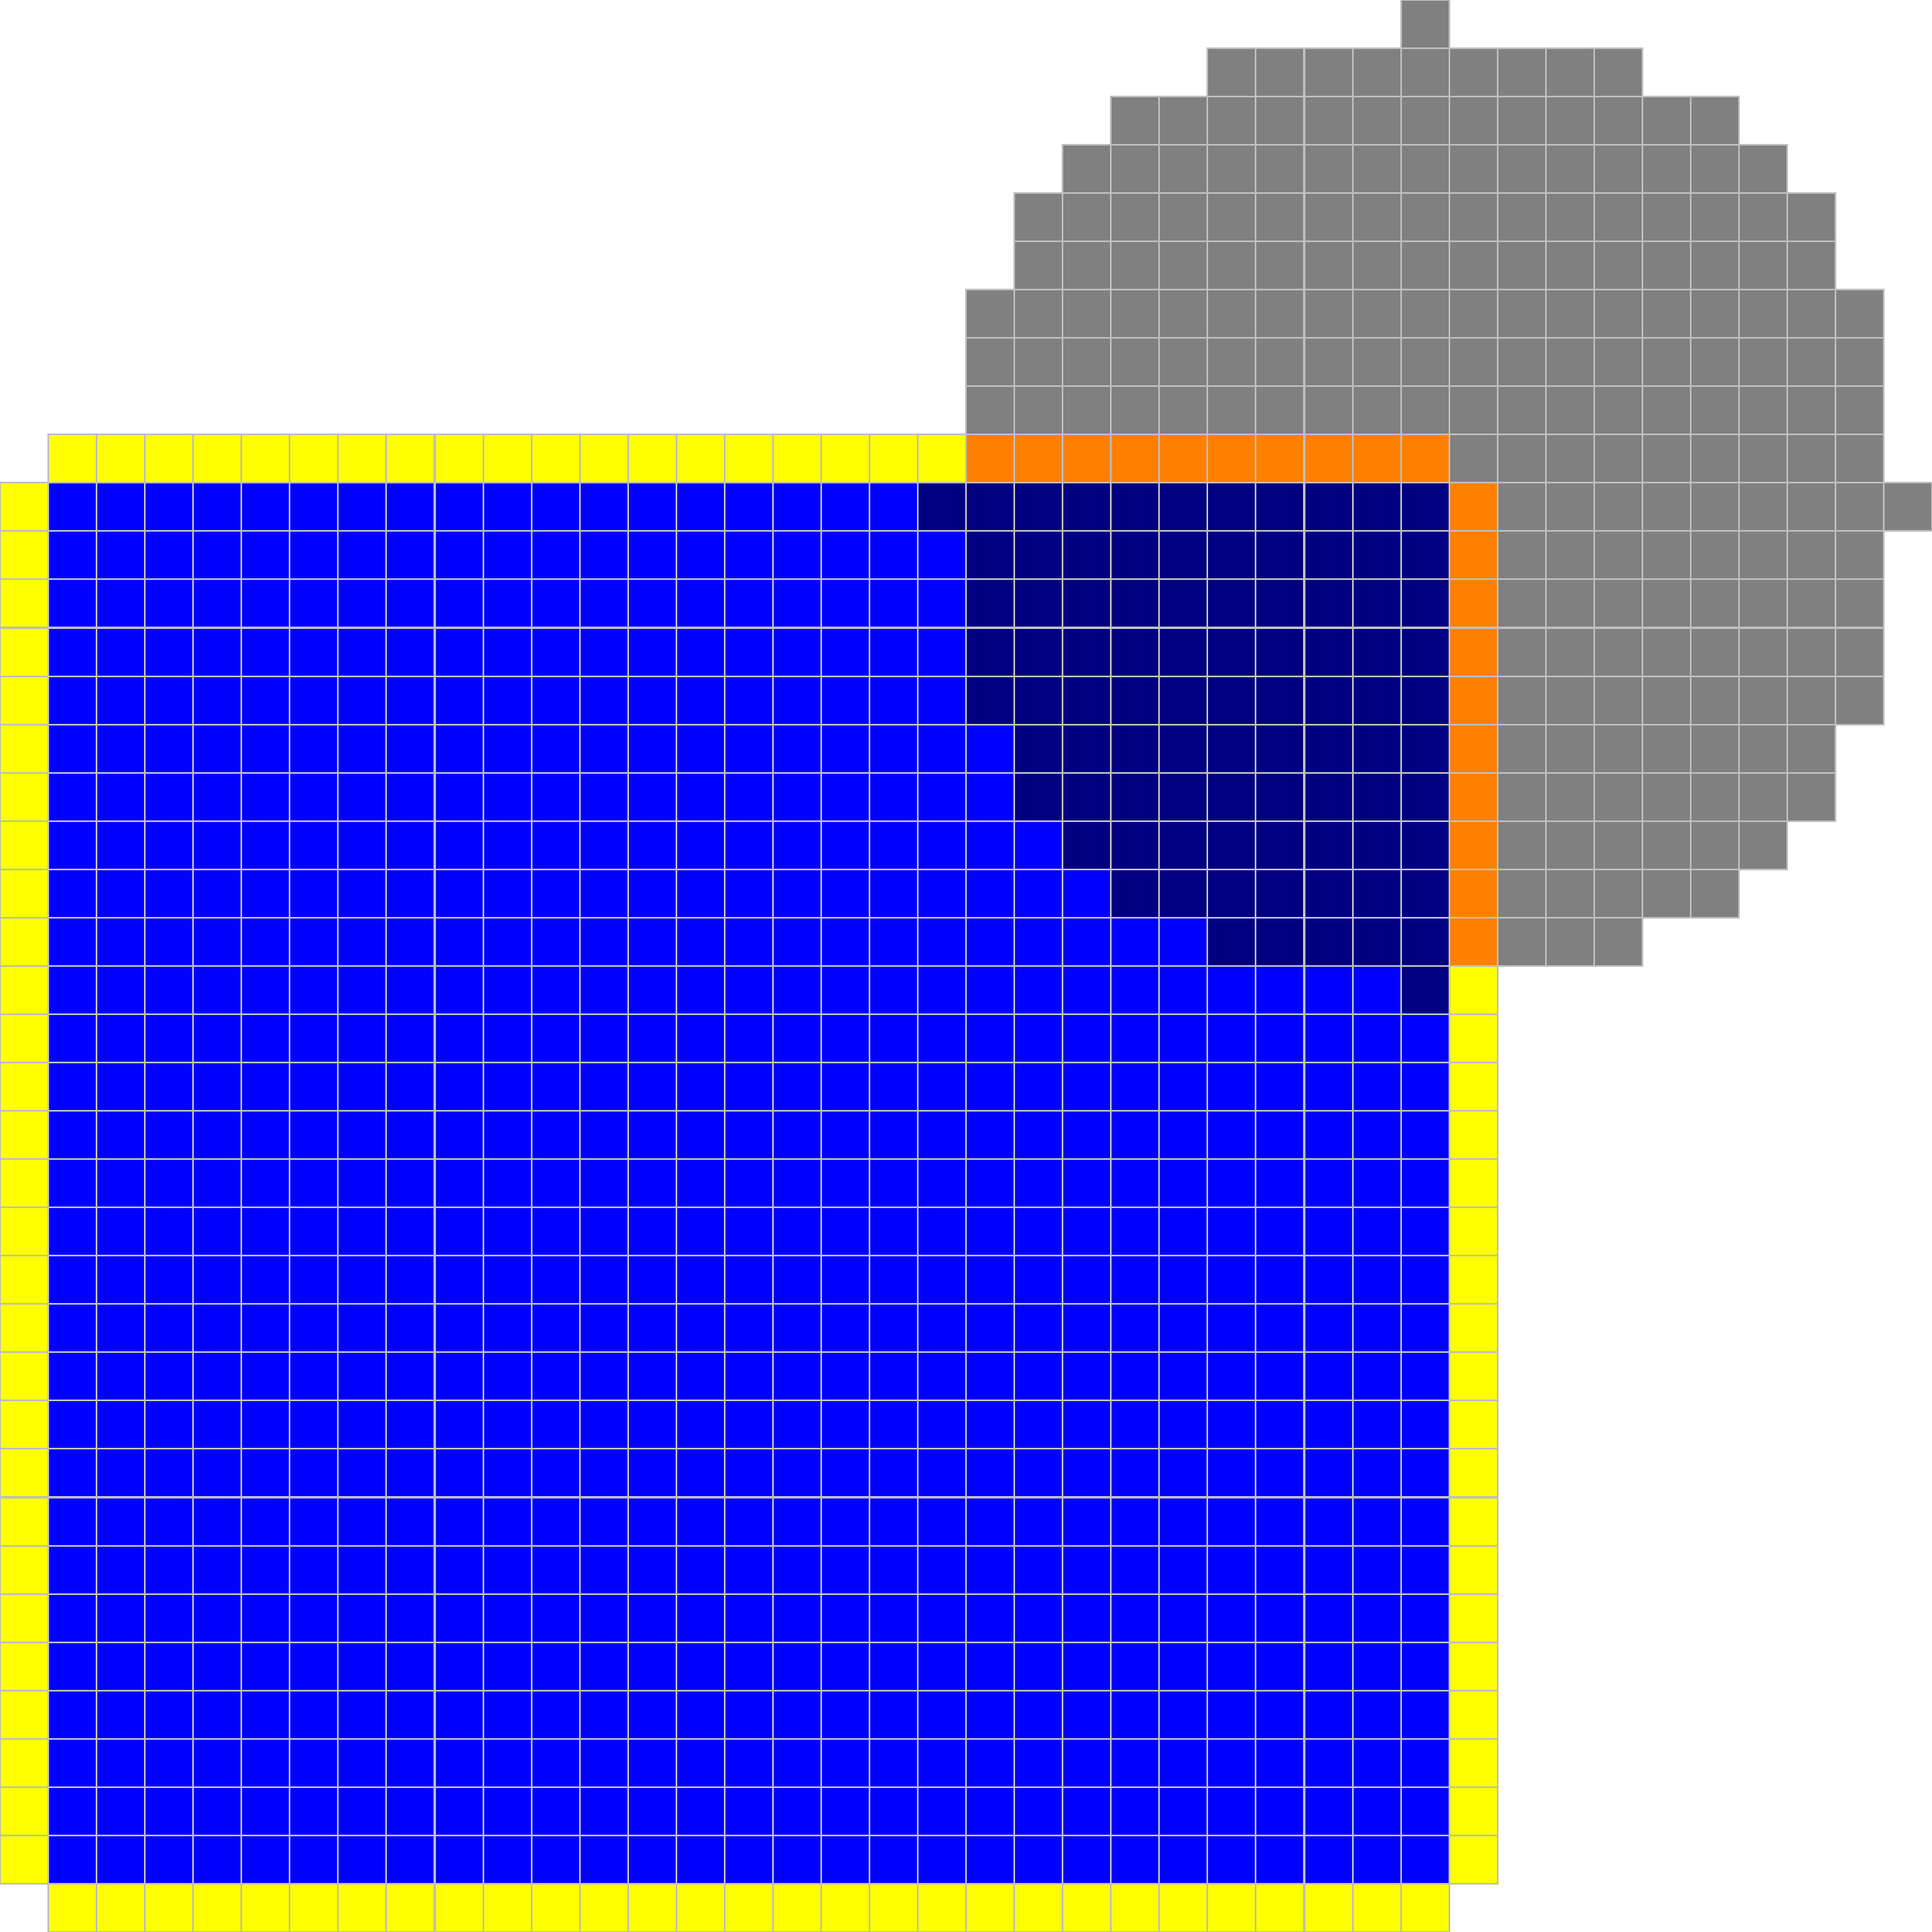
\includegraphics[scale=0.18]{figures/chapter6/contour-information/before-opt.pdf}}
\subfloat[\label{fig:naive-opt-after}]{
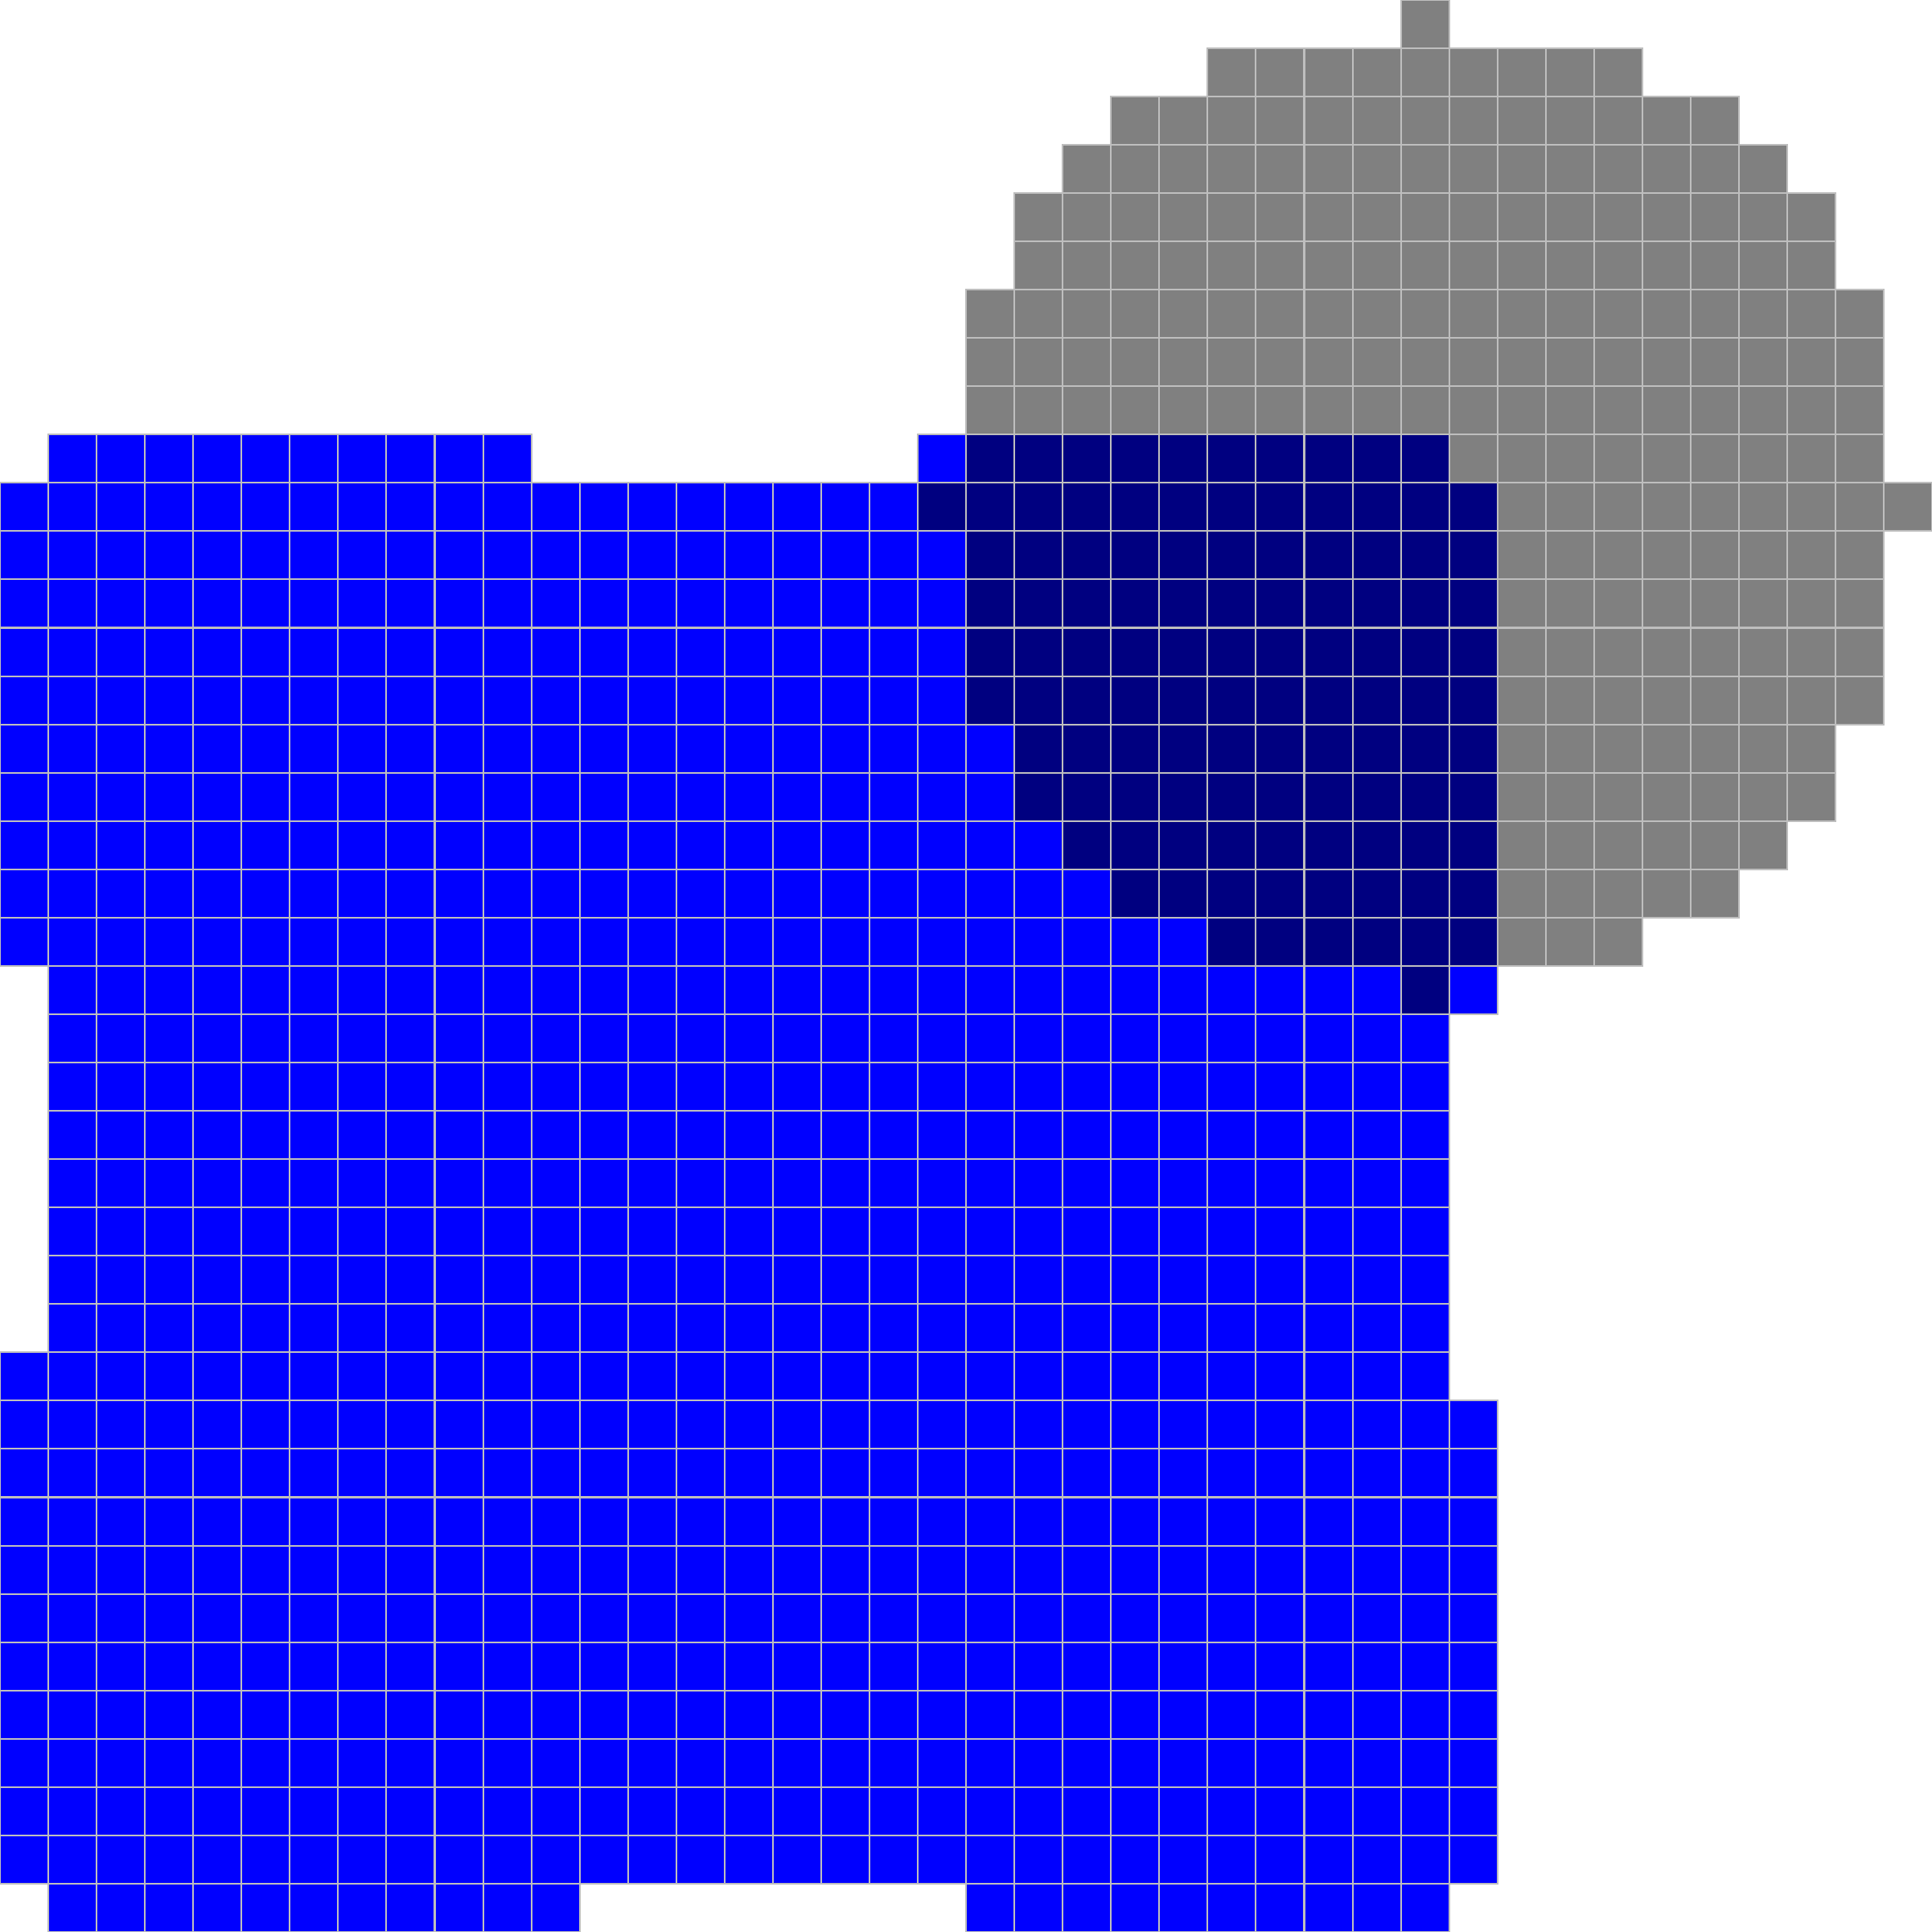
\includegraphics[scale=0.18]{figures/chapter6/contour-information/after-opt.pdf}}
\caption{Solution of model \eqref{eq:naive-opt-problem} for the square shape $(h=0.5,r=10)$. In (a) we have the square shape before minimization. Optimization variables are colored yellow. In (b), the resulting shape of the optimization problem. }
\label{fig:naive-opt-problem}
\end{figure}

The solution in figure \ref{fig:naive-opt-after} should not cause any surprise. The energy \eqref{eq:naive-opt-problem} is optimized over a fixed contour, i.e., independently of pixels being labeled zero or one the estimation ball is evaluated at the same initial contour. In section \ref{sec:global-optimization-model} we've defined an optimization energy in which contour information is taken into account, but we end up with a difficult optimization problem.

Nonetheless, we can exploit the II estimator definition to derive an energy which the minimization will lead to a shape with lower digital elastica value.


\begin{definition}{Unbalance coefficent}
Given digital shape $S \in \Omega$, positive number $r$ and point $p \in \Omega$, the \emph{unbalance coefficient} of $S$ at $p$ is defined as

\begin{align*}
	u(p) = \left( \frac{\pi r^2}{2} - |B_r(p) \cap S| \right)^2.
\end{align*}

\end{definition}

The unbalance coefficient definition is very similar to the II curvature estimator, except by the scaling factor $\frac{3}{R^3}$ and that the unbalance coefficient is defined everywhere and not only on the shape boundary.

The unbalance coefficient is used to estimate the effect of moving the estimation ball center towards the interior or the exterior of the shape. For example, consider the figure \ref{fig:unbalance-plot} in which we plot the unbalance coefficients of points along the diagonal of a square shape. 

\begin{figure}[h!]
\center
\begin{minipage}{0.25\textwidth}
\subfloat{
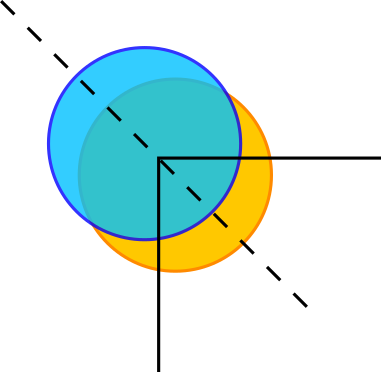
\includegraphics[scale=1.0]{figures/appendix-potential-elastica/distant-disks-1.png}}\\%
\subfloat{
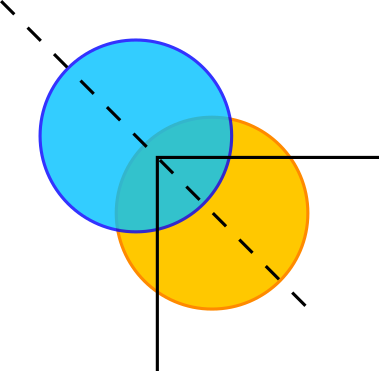
\includegraphics[scale=1.0]{figures/appendix-potential-elastica/distant-disks-2.png}}\\%
\subfloat{
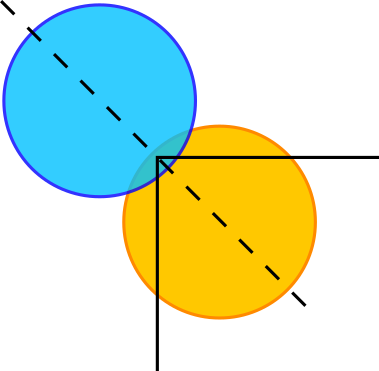
\includegraphics[scale=1.0]{figures/appendix-potential-elastica/distant-disks-3.png}}
\end{minipage}%
\begin{minipage}{0.75\textwidth}
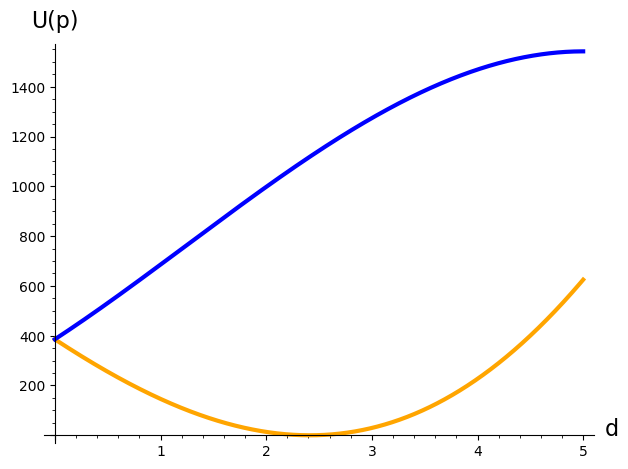
\includegraphics[scale=0.75]{figures/appendix-potential-elastica/potential-elastica-plot.png}
\end{minipage}
\caption{The unbalance difference of equidistant points from the shape contour preserves squared curvature information.}
\label{fig:unbalance-plot}
\end{figure}


We observe that the unbalance grows if the estimation ball is moved towards the exterior and decreases if the estimation ball is moved towards the interior of the shape. That is an indication that we should remove point $p$ from $S$ to decrease the curvature of the shape at point $p \in \partial S$. 


\section{Formalization}

Let $r>0,k \in \mathbb{R}$. For any point $p \in I(S)$, define

\begin{align*}
	c_{r,k}(p) = k\vec{n}(p).
\end{align*}

To simplify notation, we assume $r,k$ are fixed positive values and we denote $c_j^- = c_{r,-k}(x_j)$ and $c_j^+ = c_{r,k}(x_j)$. We define the energy

\begin{align*}
	E() &= \sum_{x_j}{ x_j (\, u(c_j^+) - u(c_j^-)\, )}
\end{align*}

\begin{definition}{k-potential}
Given digital shape $S$, natural numbers $r>0, k \neq 0$, the \emph{k-potential} at point $p$ is defined as

\begin{align*}
	U_{S,k}(p) &= \sum_{q \in Q(p)}{ u(q),}
\end{align*}

where its zone of influence $Q(p)$ is defined as

\begin{align*}
	\mathcal{Q}(p) &= \left\{\; p \in B_r(q) \; \right\}.
\end{align*}

\end{definition}

\begin{figure}[h!]
\center
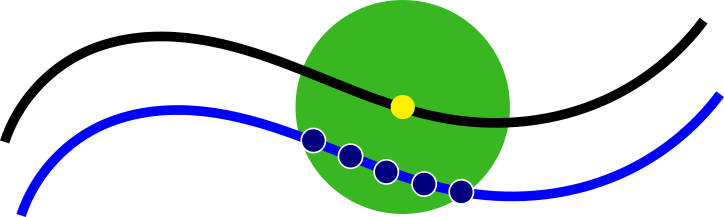
\includegraphics[scale=0.5]{figures/appendix-potential-elastica/k-potential.png}
\caption{The blue points forms the interference set of the yellow point.}
\label{fig:unbalance-set}
\end{figure}

The interference set of $p$ is the set of all points $q$ in which $p$ is contained in the estimation ball centered at $q$.   







The k-potential is used to decide which pixels are to be removed or to be kept in the next shape of the flow. 


\begin{definition}{$k$-flow}
	Given digital shape $X$, we define its $k$-flow as
	
	\begin{align*}
		F_k = \Big\{& S^{(i)} \; | \\
			& S^{(0)} = S,\\
		    &S^{(i+1)} = \argmin \sum_{ x_j \in X(I(S^{(i)}))}{ x_j \Delta _j\big(\; U_{S,k}(p) - U_{S,-k}(p) \;\big)} - \phi(S^{(i)},k,x_j) \; \Big\},
	\end{align*}
	
	where $\phi(S^{(i)},k,x_j)$ accounts for pairwise terms that were counted twice.
	
	\begin{align*}
	\phi(S^{(i)},k,x_j) = \frac{x_j}{2}\sum_{ x_l \in X(I(S^{(i)}))}{x_l \Delta _{jl}\big(\; U_{S,k}(p) - U_{S,-k}(p) \;\big)} 
	\end{align*}
     	  
\end{definition}	

In other words, the pixel is labeled zero (one) if its outer (inner) potential is bigger than its inner (outer) potential.

[Results for triangle, square, flower, bean. Non uniform. Balls positioned at radius-2]


We have two issues to tackle. 
\begin{enumerate}
	\item{Why the estimation balls should be centered at distant levels?}
	\item{Why the flow tends to shrink the shape?}
\end{enumerate}


\section{Distant balls}
	The optimization process performs the better when the estimation balls are positioned at distance that maximize the gap between the outer and inner unbalance. Surprisingly, this gap is independent of the curvature value in the boundary. In the experiments, we observe that the highest gap is invariably at $\frac{2}{3}$ of the estimation ball radius.
	
	The reasoning for distance balls is two fold. First, we need at least a $k=1$ in order to compute the unbalance, otherwise it would be zero. The question is how large should be $k$? The energy is easier to optimize if the gap between outer and inner curves is at its maximum. We should find a compromise value for $k$ that assure us a sufficiently large gap. 
	
	Second, the inner and outer balls estimates the impact of shifting the center of the ball from a single point in the boundary. That means that limiting the region of influence of each pair of inner and outer balls is important.
	
	Each pair of inner and outer balls evaluates the shifting of a single point in the boundary.
	
	We do not impose any mapping between the inner and outer balls. It will be too complicated. And we don't need to do it. The mapping is somehow implicitly defined by the distance level curves. 
	
	However, the closer the balls are from the boundary the bigger it is its zone of influence. Ideally, we should set weigths for each pixel in the ball accordingly to its distance from the normal. This is also complicated! 
	
	Nonetheless, there is a natural way to implement that. If the balls are in distant levels, its zone of influence englobes a small area around the normal. We've got the weighting by normals for free!
	
	
	
	

\section{Controlling the shrinking}

\section{Unbalance plot development}
	The unbalance difference at a point $c \in S$ distant $d$ units from the corner is written as
	\begin{align*}
		u_i(c) &= \frac{\pi r^2}{2} - \big( \; a^2 + area( APC ) + area(A'PC) + area(\arc{PQ})  \; \big) \\
		&= \frac{\pi r^2}{2} - \big( \; a^2 + a(P_x-a) + \frac{\theta_P + \theta_Q + \pi/2}{2\pi} \pi r^2\; \big),
	\end{align*}
	
	where
	
	\[
	\begin{array}{ll}
	a = d\sqrt{1/2} & \theta_P = \arctan \frac{a}{P_x-a} \\		
	Q_y = -P_x = a + \sqrt{r^2 -a^2} & \theta_Q = \arctan \frac{a}{|Q_y|-a}		
	\end{array}\]
	
%default = pi*R^2*(abs(t2) + abs(phi))/(2*pi) + a*abs(p2[0])

%g2 = pi*R^2/2 - ( pi*R^2 - ( pi*R^2/4 - default) )	
	
	Similarly, for the outer ball
	\begin{align*}
		u_o(c) &= \frac{\pi r^2}{2} - \big(\; \frac{\pi r^2}{4} - area(APC) - area(AQC) - area(\arc{CP'}) - area(\arc{CQ'}) \; \big)\\
		&= \frac{\pi r^2}{2} - \big( \; \frac{\pi r^2}{4} - aP_x - \frac{\theta_P + \theta_Q}{2\pi}\pi r^2 \; \big),
	\end{align*}
	
	where
	\[
	\begin{array}{ll}
		a = d\sqrt{1/2} & \theta_P = \arctan \frac{a}{P_x+a}\\
		Q_y = -P_x = \sqrt{r^2-a^2} - a & \theta_Q = \arctan \frac{a}{|Q_y|+a}
	\end{array}	 \]
	
\begin{figure}[h!]
	\begin{minipage}{0.5\textwidth}
	\center
	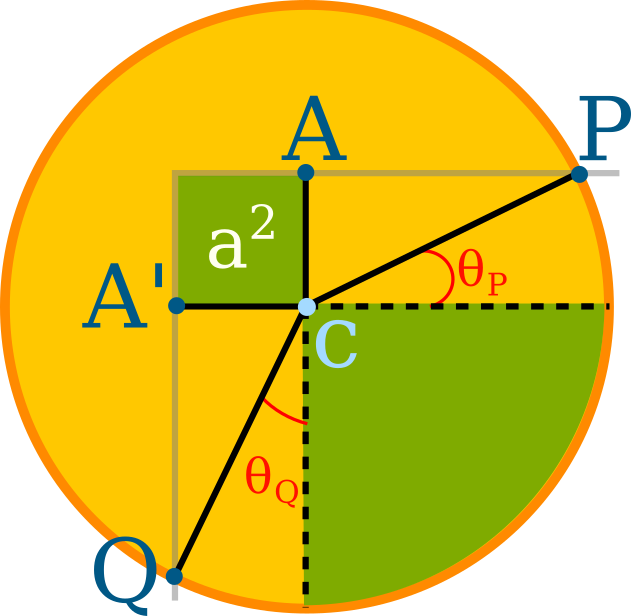
\includegraphics[scale=2.0]{figures/appendix-potential-elastica/balance-dev-1.png}
	\end{minipage}%
	\begin{minipage}{0.5\textwidth}
	\center
	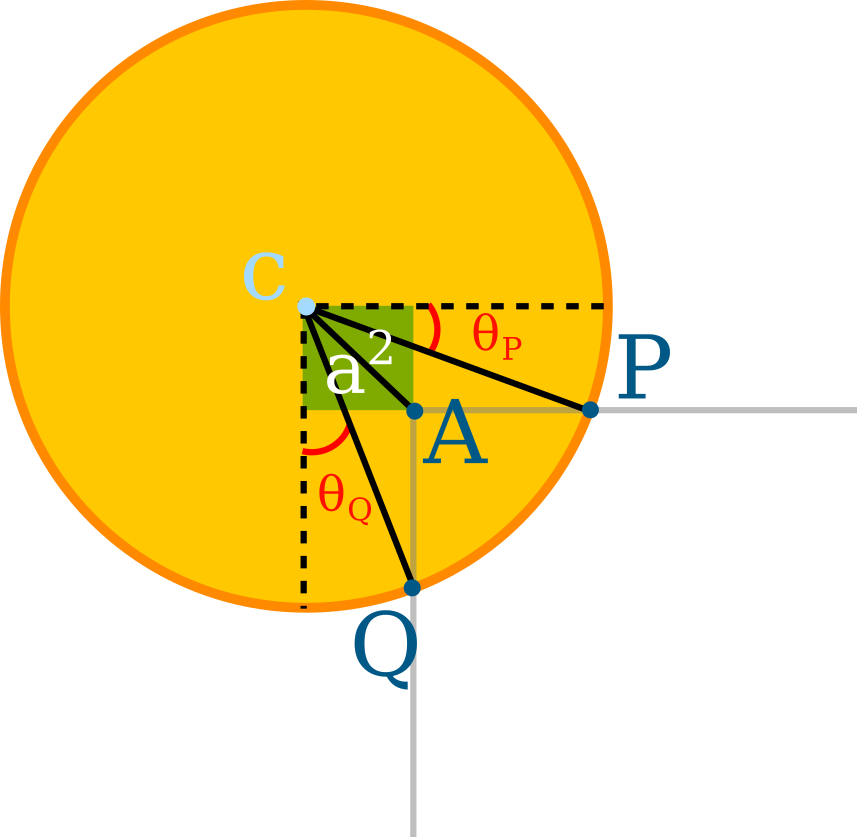
\includegraphics[scale=2.0]{figures/appendix-potential-elastica/balance-dev-2.png}
	\end{minipage}	
\end{figure}
